\section{Model Overview}



In order to solve those problems, we will proceed as follows:

\begin{itemize}
    \begin{figure}[htbp]
        \centering
        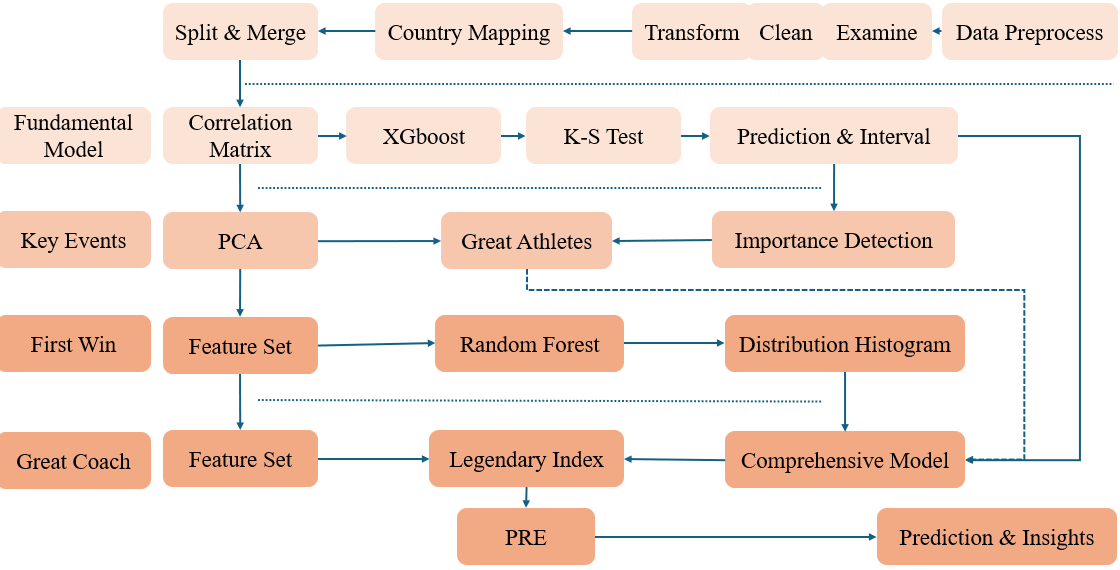
\includegraphics[width=0.8\textwidth]{./figures/figure1_work_flow.png}
        \caption{Figure1 Flow chart of our work}
        \label{fig:example}
    \end{figure}
    
\item {\bf Stating assumptions}. By stating our assumptions, we will narrow the focus of our approach towards the problems and provide some insight into Olympic medal issues.

\item {\bf Making notations}. We will give some notations which are important for us to clarify our models.

\item {\bf Presenting our model}. In order to investigate the problem deeper, we divide our model into three sub-models. One is a \textbf{medal tally} prediction model based on past data and host country effect. 
Another one is a non-linear model focusing on the analysis of data characters of the relevant period when a country won its \textbf{first} medal.
The last is about certain \textbf{key sports/events}, \textbf{great coach} and \textbf{great athletes}

\item {\bf Defining evaluation criteria and comparing sub-models}. We define two main criteria to evaluate our model: the precision of our model and the ability to calculate probability of winning first medal.

\item {\bf Analysis of influencing factors}. In term of the impact of different factors on our model, we take those into consideration:
medal tally, year and participation.

\item {\bf Model testing and sensitivity analysis}. With the criteria defined before, we evaluate the reliability of our model and do the sensitivity analysis.

\item {\bf Further discussion}. We discuss about different ways to arrange medal counts. Then we improve our model to apply them in reality.

\item {\bf Evaluating the model}. We discuss about the strengths and weaknesses of our model:

\begin{itemize}
\item[1)] ... 
\item[2)] ...
\item[3)] ...
\item[4)] ...
\end{itemize}

\end{itemize}
